% LaTeX formatting example for NERCCS
% Revised on 11/07/2020 by Dane Taylor

\documentclass[12pt]{article}
\usepackage[letterpaper,margin=1in]{geometry}
\usepackage{times}
\usepackage{graphicx}
\usepackage{sectsty}
\allsectionsfont{\normalsize}
\usepackage{authblk}
\renewcommand\Authfont{\normalsize}

\begin{document}

\title{\normalsize\bf \vspace{-8ex}
LaTeX Formatting Example for NERCCS 2020}

\author{Jane Doe$^1$ and John Doe$^2$\\
$^1$ Center for Collective Dynamics of Complex Systems\\
Binghamton University, State University of New York\\
janedoe@coco.binghamton.edu\\
$^2$ Center for Singular Dynamics of Simple Systems\\
Binghamton University, State University of New York\\
johndoe@sisi.binghamton.edu}

\date{\vspace{-5ex}} % to kill the unnecessary blank space for \date{}

\maketitle

\thispagestyle{empty}
\pagestyle{empty}


Write your extended abstract here.  See the NERCCS formatting instructions \cite{nerccsinstructions} for more details. References should be included in full papers (but are not required for extended abstracts).  References should be sorted in the order they appear in the text.  One figure is required in extended abstracts. Multiple figures and tables are allowed in full papers. Color figures may be used. Figure \ref{fig:sinx} shows a sine wave plotted over the domain $[0,10]$.

If you have any questions, email danet@buffalo.edu.


\begin{figure}[h]
\centering
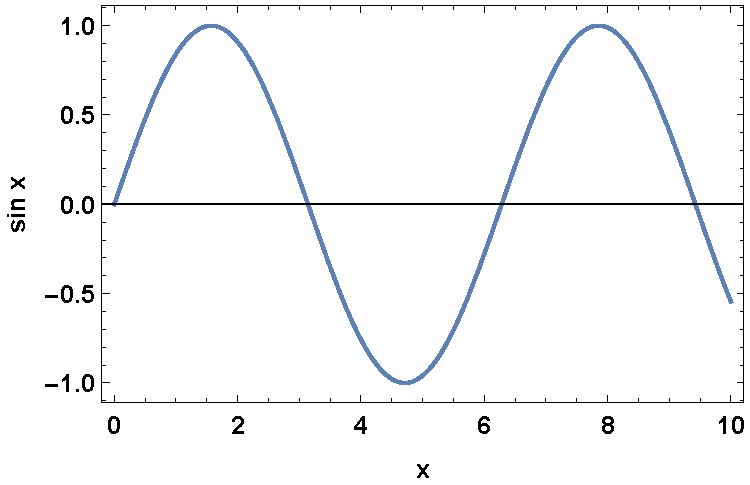
\includegraphics[width=0.5\columnwidth]{fig1.pdf}
\caption{A sine wave plotted over $[0,10]$.}
\label{fig:sinx}
\end{figure}

 
\begin{thebibliography}{99}
\bibitem{nerccsinstructions} TBD
\end{thebibliography}

\end{document}